
\documentclass[a4paper]{article}
\usepackage{color}
\usepackage{url}
\usepackage[utf8]{inputenc}
\usepackage{graphicx}
\usepackage{tabu}
\usepackage{float}
\usepackage{tcolorbox}
\usepackage{titlesec}
\usepackage{biblatex}

\usepackage[english,serbian]{babel}





\usepackage[unicode]{hyperref}
\hypersetup{colorlinks,citecolor=green,filecolor=green,linkcolor=blue,urlcolor=blue}


\def\d{{\fontencoding{T1}\selectfont\dj}}
\def\D{{\fontencoding{T1}\selectfont\DJ}}




\begin{document}

\title{\textbf{KLASTEROVANJE GENA}\\ \small{Seminarski rad u okviru kursa\\Istraživanje podataka 2\\ Matematički fakultet, avgust 2019.}}


\author{Darko Veizović, 310/2015 \\ \\ \\ \\ \\ \\ }
\date{}
\maketitle

\\
\\
\\
\\
\\

\tableofcontents
 



\\
\\
\\
\\
\newpage






\section{Uvod}
\label{sec:uvod}
\textbf{Istraživanje podataka} predstavlja proces otkrivanja korisnih informacija u skupovima podataka. Tehnike koje se koriste pretražuju podatke u cilju pronalaska neobičnih i korisnih obrazaca. 
\textbf{Klasterovanje} je jedna od tehnika istraživanja podataka koja za cilj ima pronalaženje objekata sličnih osobina i njihovu podelu u grupe, odnosno klastere, čineći ih tako preglednijim i upotrebljivim.
\\
Rad predstavlja prikaz različitih tehnika i algoritama klasterovanja koji su korišćeni za istraživanje podataka na primeru baze podataka o ćelijama. Za obradu podataka korišćeni su programski jezici \textbf{C++}, \textbf{Python} i \textbf{R}, kao i softver \textbf{Orange}.
Upotrebljene su različite metode klasterovanja, a u nastavku su iste detaljno obrazložene.
 
\\


\section{Opis skupa podataka}
 

Izvorna datoteka naziva \textbf{005\_Lymphoblastoid\_cell\_line\_GM12891\_csv.csv} sadrži podatke o \textbf{limfoblastičnim ćelijama(LCL)}. Naime, izolovanje DNK materijala korak je koji ograničava brzinu istraživanja, postojanje LCL ćelija koje predstavljaju surogat izolovanim perifernim krvnim ćelijama značajno ubrzava proces bioloških ispitivanja. LCL ćelije mogu se izdvojiti \textit{in vitro} infekcijom perifernih B-ćelija, što rezultira kontinuiranim izvorom, podnoseći zanemarljive fenotipske i genotipske promene. Budući da postoji spontani izvor razmnožavanja, LCL ispunjava zahtev za stalnim snabdevanjem polaznim materijalom za različite testove, štedeći potrebu za ponovnim uzorkovanjem.
Postoji razlog za verovanje da su LCL u bliskoj srodnosti sa matičnim limfocitima na osnovu obimnih potpornih opažanja iz različitih studija koja pokazuju značajan nivo korelacije na molekularnom i funkcionalnom nivou. LCL ćelije, koje nose kompletan set genetskog materijala iz klice, bile su generalno instrumentalni izvor biomolekula i sistem za sprovođenje različitih imunoloških i epidemioloških ispitivanja. Štaviše, u novije vreme njihova upotreba za analizu celokupnog ljudskog genoma opširno je dokumentovana. Ovo dokazuje korisnost LCL-a u raznim genetičkim i funkcionalnim studijama. Postoji nekoliko kontradiktornih izveštaja koji dovode u pitanje zapošljavanje LCL-a kao roditelja surogata. Bez obzira na neka svojstvena ograničenja, LCL se sve više smatraju važnim resursom za genetička i funkcionalna istraživanja.
\\

Ulazni materijal sadrži rezultate istraživanja skupova različitih humanih ćelija.
Ulazna datoteka sadrži podatke vezane za ekspresiju \textbf{31221} gena. Nazivi svih gena imaju prefiks \textit{hg38} koji označava da su
podaci vezani za verziju 38 humanog genoma.  

\begin{figure}[H]
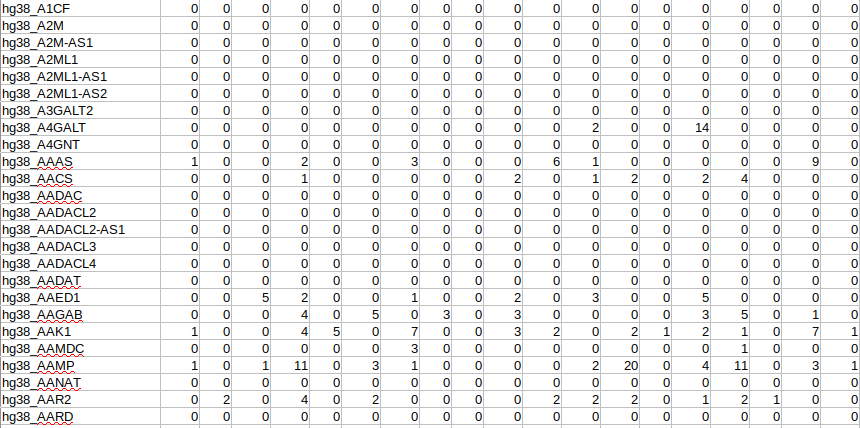
\includegraphics[width=12cm]{images/dataSet.png}}}}}}
\caption{primer podataka}
\end{figure}
 
Ulazna datoteka sadrži podatke u CSV formatu u obliku ukrštene tabele (podatak
u preseku prvog reda i prve kolone je prazan). Datoteka ima \textbf{31221} red i
\textbf{6484} kolone, pri čemu prvi red sadrži redni broj ćelije za koju je vršeno istraživanje, a prva kolona sadrži identifikaciju gena. 

 
\section{Priprema podataka}
\label{sec:naslov1}
U okviru istraživanja podataka, ključna uloga pripada podacima, stoga određivanje istih sa pogodnim osobinama za dalju obradu, jeste prvi korak u procesu klasterovanja. Na prvi pogled, može se učiniti da podaci imaju pogodne osobine, međutim u stvarnosti oni sa sobom nose mnoštvo problema. Proces \textbf{pretprocesiranja} podataka predstavlja skup tehnika kojima se dobijaju pogodni podaci koji će kasnije predstavljati ulazni skup za algoritme klasterovanja. Izvorni skup podataka uglavnom mora biti podvrgnut pretprocesiranju kako bi postao pogodniji za dalju analizu. Programi za pretprocesiranje pisani su u programskom jeziku \textbf{C++}, a kao rezultat imali su prilagođavanje podataka konkretnim tehnikama i alatima za klasterovanje.
\\
\subsection{Uklanjanje nultih redova}
\begin{figure}[H]
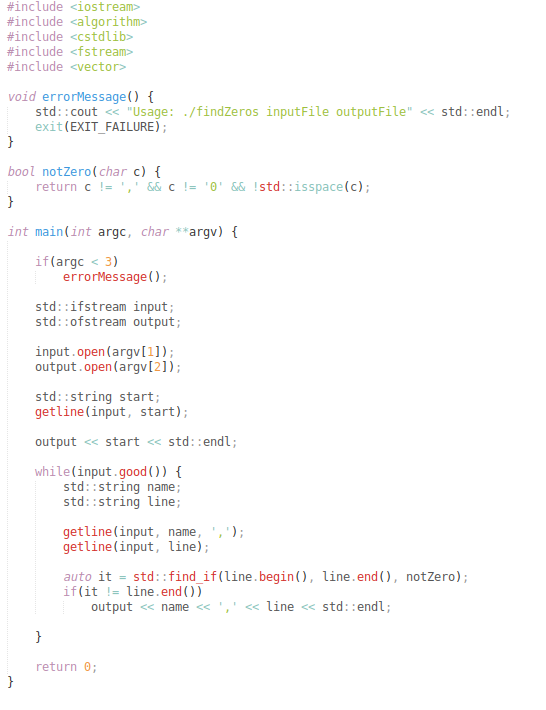
\includegraphics[width=12cm]{images/findZerosCpp.png}}}}
\caption{findZeros.cpp}
\end{figure}  

U našem slučaju, ulazna datoteka sadržala je veliki broj redova, tj. gena koji su za svaku od 6383 ćelije, kao numeričku reprezentaciju iste imali vrednost - \textbf{0}. Kako ovako definisani geni ne bi imali uticaj na proces klasterovanja, a njihovim izbacivanjem iz dalje obrade isti bi bio značajno efikasniji, pomenuti geni uklonjeni su iz skupa podataka.
\\
 \\

Prevođenje programa potrebno je izvršiti komandom:
\begin{tcolorbox}
\begin{verbatim}
g++ findZeros.cpp -o findZeros 
\end{verbatim}
\end{tcolorbox}

nakon čega se isti pokreće izvršavanjem naredbe:

\begin{tcolorbox}
\begin{verbatim}
./findZeros inputFile outputFile
\end{verbatim}
\end{tcolorbox}

 
 
Pre uklanjanja nultih gena, broj redova bio je \textbf{31221}, dok se nakog istog taj broj smanjio na \textbf{10561}. Ovakva redukcija značajno utiče na efikasnost samih algoritama. Algoritmi klasterovanja su u najvećem broju slučajeva kvadratne složenosti, pa se smanjivanjem skupa podataka dobija na brzini i vremenu izvršavanja. Ovako pripremljen skup podataka biće ulaz za sve navedene algoritme klasterovanja, uz izvesna prilagođavanja.

 
\subsection{Transponovanje podataka}
Ovako pripremljeni podaci, pogodni su za klasterovanja na osnovu gena. Međutim, klasterovanje na osnovu ćelija zahteva nešto drugačiji ulazni skup. Naime, da bi se podaci klasterovali na osnovu ćelija, neophodno je najpre transponovati iste, tako da ćelije predstavljaju redove u tabeli, dok geni popunjavaju kolone.
Program koji transponuje podatke, napisan je u programskom jeziku \textbf{C++}, pri čemu je korišćena biblioteka \textbf{boost}.

 
\begin{figure}[H]
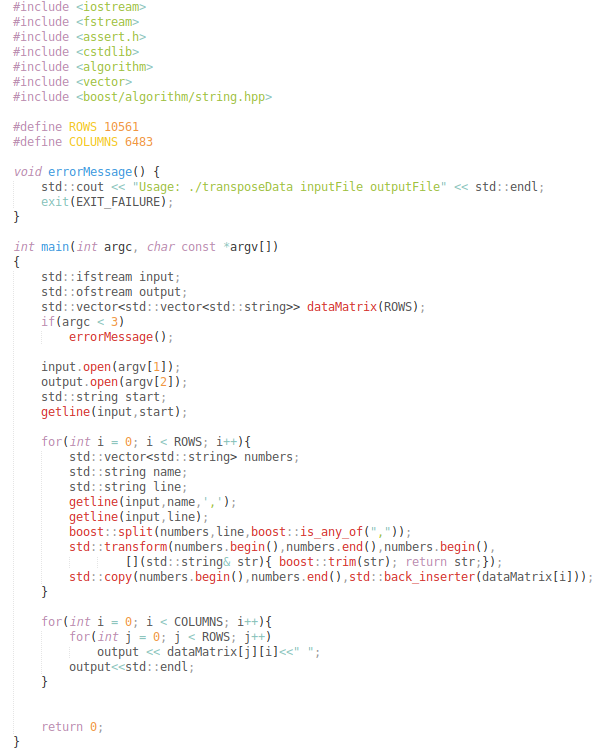
\includegraphics[width=12cm]{images/transposeDataCpp.png}}}}
\caption{transposeData.cpp}
\end{figure}  

\\

Prilikom prevođenja programa neophodno je proslediti putanju do boost biblioteke na sledeći način:
\begin{tcolorbox}
\begin{verbatim}
g++ transposeData.cpp -o transposeData - I /path/to/boost/
\end{verbatim}
\end{tcolorbox}


\section{Orange}
\textbf{Orange} je open-source softver za mašinsko učenje, vizualizaciju i istraživanje podataka. Razvijen je 10. oktobra 1996. godine od strane Univerziteta u Ljubljani. Softver je pisan na programskim jezicima C++, Python i C, a slobodan je u upotrebi ili uz grafički-korisnički interfejs ili kao spoljašnja biblioteka jezika Python. Dostupan je za operativne sisteme \textit{Linux}, \textit{Windows} i \textit{Mac}.


 
\begin{figure}[H]
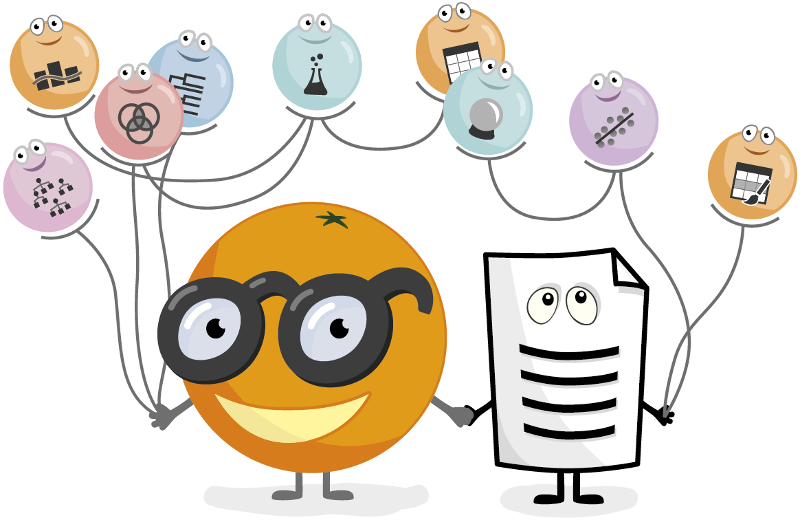
\includegraphics[width=12cm]{images/orange.png}}}}
\caption{orange}
\end{figure}  

Instalacija \textbf{Orange} softvera na operativnom sistemu \textit{Linux} može se izvršiti pozivom sledećih komandi iz komandne linije.

\begin{tcolorbox}
\begin{verbatim}
sudo apt install virtualenv build-essential python3-dev
\end{verbatim}
\end{tcolorbox}

\begin{tcolorbox}
\begin{verbatim}
virtualenv --python=python3 --system-site-packages orange3venv
\end{verbatim}
\end{tcolorbox}


\begin{tcolorbox}
\begin{verbatim}
pip install PyQt5 PyQtWebEngine
\end{verbatim}
\end{tcolorbox}

\begin{tcolorbox}
\begin{verbatim}
pip install orange3
\end{verbatim}
\end{tcolorbox}

\\
\\

Pokretanje programa moguće je komandom:

\begin{tcolorbox}
\begin{verbatim}
orange-canvas
\end{verbatim}
\end{tcolorbox}

ili

\begin{tcolorbox}
\begin{verbatim}
python3 -m Orange.canvas
\end{verbatim}
\end{tcolorbox}

\subsection{K-means}

\subsubsection{Klasterovanje gena}

Za učitavanje podataka iskorišćen je čvor \textbf{CSV File Import}. Učitani su unapred pripremljeni podaci, odnosno skup podataka kome su uklonjeni nulti redovi, stoga je ukupan broj redova 10561 od kojih svaki sadrži osobine odgovarajućeg gena.
Čvor \textbf{k-Means} koji se koristi za proces klasterovanja podešen je tako da softver sam odredi optimalan broj klastera. Pre određivanja broja klastera, pokušalo se sa klasterovanjem podataka za različit broj klastera, pri čemu se zaključilo da za broj klastera veći od 8 podaci nisu dobro raspoređeni, stoga je programu prosleđen fiksiran interval u kom traži optimalan broj klastera, odnosno interval od 2 do 8. Maksimalan broj iteracija postavljen je na 300.

\begin{figure}[H]
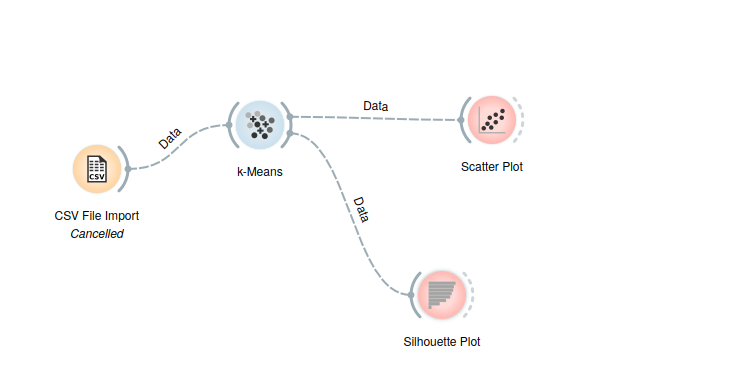
\includegraphics[width=12cm]{images/orange1.png}}}}
\caption{algoritam Kmeans}
\end{figure}  

Pomoću čvora \textbf{Scatter plot} vizualizovani su dobijeni klasteri.

\begin{figure}[H]
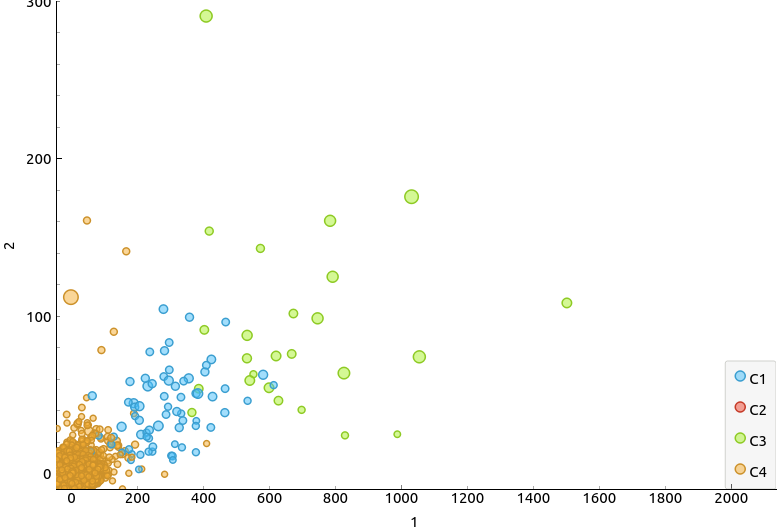
\includegraphics[width=12cm]{images/kmeans_4clusters.png}}}}
\caption{vizualizacija dobijenih klastera}
\end{figure}  

Sa slike se može zaključiti, da se uz ovako podešene parametre za klasterovanje metodom K-means, kao optimalan broj klastera izdvaja 4. Podaci su neravnomerno raspoređeni u klastere, takođe gustina klastera se izuzetno razlikuje. U okviru jednog klastera grupisana je većina podataka, dok preostala tri klastera sadrže neznatan broj istih. Te stoga možemo zaključiti da ovakvom metodom nismo uspeli da valjano klasterujemo ulazni skup podataka. Silueta rastojanja između klastera data je u direktorijumu \textbf{clusters} u vidu slike odgovarajućeg naziva.


\begin{figure}[H]
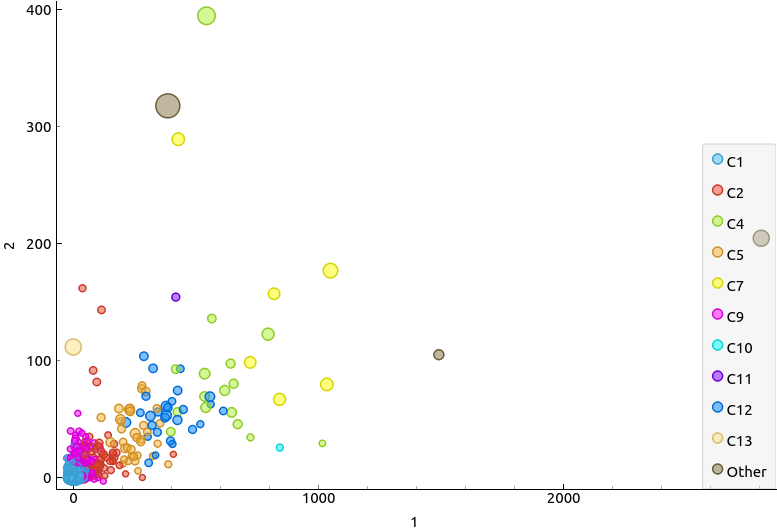
\includegraphics[width=12cm]{images/kmeans.png}}}}
\caption{vizualizacija dobijenih klastera}
\end{figure}  

Promenom ulaznih parametara algoritma, odnosno fiksiranjem broja klastera na 13 nisu dobijeni značajno bolji rezultati. Klasteri su nešto ujednačenijih veličina, međutim podaci ponovo nisu kvalitetno raspoređeni. Uočeno je veće preklapanje među grupisanim podacima, takođe pronađen je i veći broj elemenata van granica. \\

\begin{tcolorbox}
\begin{verbatim}
CLUSTER0 - 71
CLUSTER1 - 1
CLUSTER2 - 27
CLUSTER3 - 10462
\end{verbatim}
\end{tcolorbox}

Raspored veličina klastera dobijen za 4 klastera. Izdvaja se klaster najveće gustine u kom se nalazi veliki deo podataka.


\subsubsection{Klasterovanje ćelija}
Prilikom klasterovanja ćelija iskorišćen je sličan postupak kao prilikom klasterovanja gena, pri čemu se za ulaznu datoteku uzima skup transponovanih podataka.
 

\begin{figure}[H]
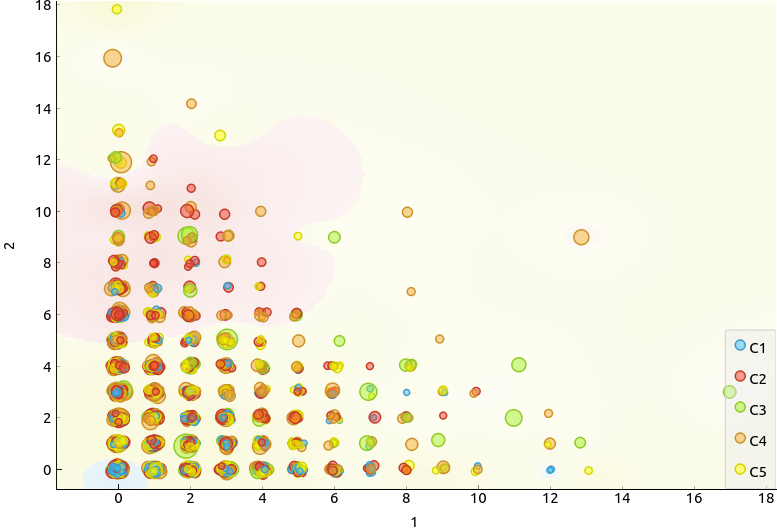
\includegraphics[width=12cm]{images/kmeans_5.png}}}}
\caption{5 klastera}
\end{figure}  
 
\begin{figure}[H]
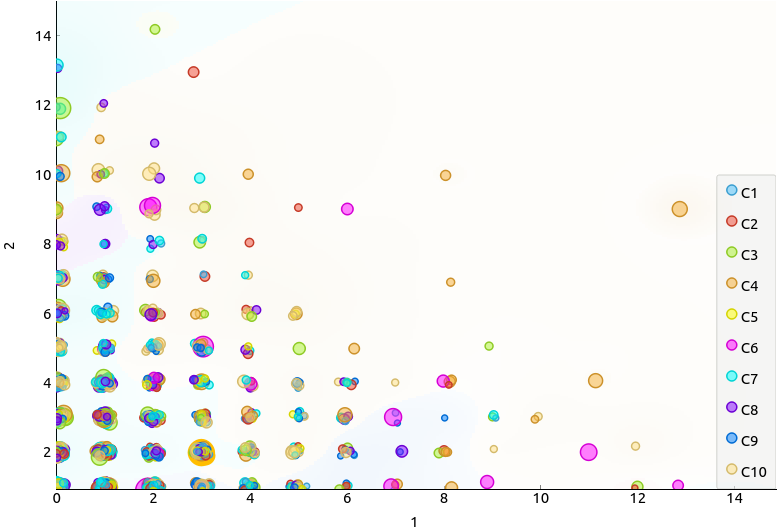
\includegraphics[width=12cm]{images/kmeans_10.png}}}}
\caption{10 klastera}
\end{figure}  




 

U ovom slučaju, pokušalo se sa različitim brojem klastera što je rezultiralo slabijim rezultatima. Podaci su grupisani u klastere tako da zbog velikog broja preklapanja sa slike nije moguće utvrditi tačan raspored klastera.

\begin{tcolorbox}
\begin{verbatim}
    C1 - 2568
    C2 - 1358
    C3 - 94
    C4 - 429
    C5 - 2078
\end{verbatim}
\end{tcolorbox}
 
Rezultati koji su dobijeni prilikom grupisanja u pet klastera jasno izdvajaju 3 klastera koja gustinom dominiraju nad ostatkom. Sa dobijene siluete, zaključuje se da postoji veliki broj podataka koji su smešteni u jedan klaster, pri čemu imaju veliku sličnost sa podacima iz drugog klastera, što zapravo potvrđuje i vizualizaciju dobijenu čvorom Scatter plot. 

  

\subsection{Hijerarhijsko klasterovanje}
Podaci su ponovo učitani pomoću čvora \textbf{CSV File Import}. Pre primene metode hijerarhijskog klasterovanja nad ulaznim podacima, čvorom \textbf{Distances} izračunata su rastojanja između datih podataka.
Prilikom klasterovanja ovim algoritmom, koriščeni su \textbf{Euklidsko}, \textbf{Menhetn} i \textbf{Kosinusno} rastojanje.


Dendrogrami koji su dobijeni različitim postavljanjem veza(\textit{single, average, complete}) i različitom dubinom sečenja stabla dati su u nastavku.

 
\begin{figure}[H]
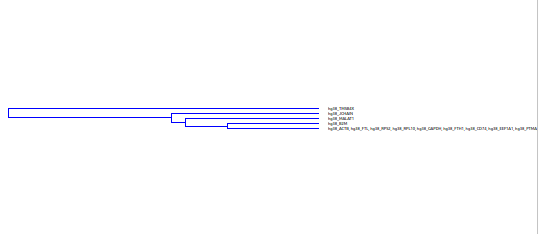
\includegraphics[width=12cm]{images/single_0.png}}}}
\caption{dendrogram1}
\end{figure}  

Rezultat dobijen pojedinačnom vezom, pri čemu nema sečenja stabla. Jasno se vidi da podaci nisu dobro raspoređeni u klastere. Postoji jedan klaster velike gustine, dok se u ostalim nalazi mali broj podataka.

 
\begin{figure}[H]
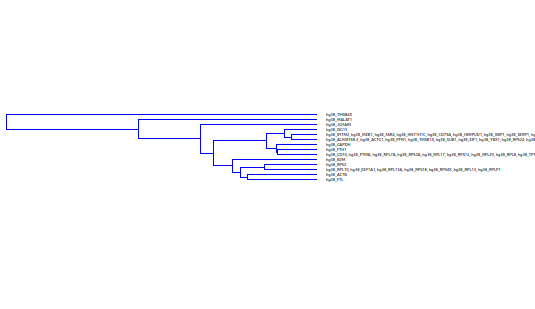
\includegraphics[width=12cm]{images/average_7.png}}}}
\caption{dendrogram2}
\end{figure}  

Prosečna veza, uz dubinu sečenja stabla - 7, dala je nešto bolje rezultate. Ovoga puta, izdvaja se grupa od nekoliko klastera koji sadrže veliku većinu podataka, sa druge strane postoje klasteri i podklasteri u kojima se nalazi neznatan broj gena.

\begin{figure}[H]
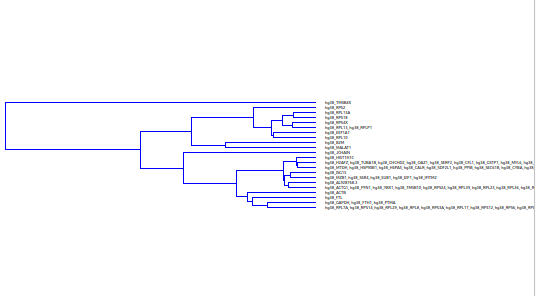
\includegraphics[width=12cm]{images/complete_7.png}}}}
\caption{dendrogram3}
\end{figure}  

 
\begin{figure}[H]
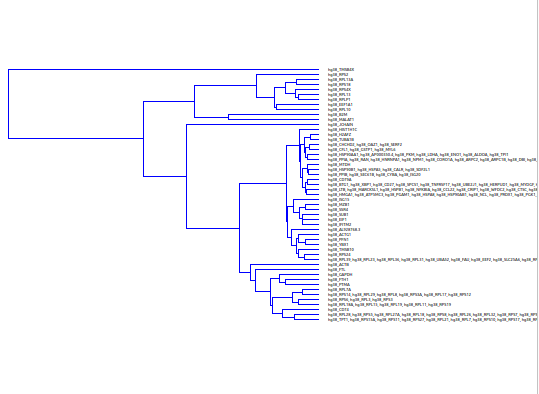
\includegraphics[width=12cm]{images/complete_10.png}}}}
\caption{dendrogram4}
\end{figure}  
 

Povećanjem dubine sečenja stabla, te različitim načinima grupisanja podklastera, moguće je povećati kvalitet klasterovanih podataka. Prilikom korišćenja različitih veza, najlošije se pokazala pojedinačna veza, dok se u slučaju prosečnog i ward povezivanja za određeni stepen ujednačuje raspored podataka u klasterima. Ipak, iz navedenih rezultata ne može se zaključiti da je ovakav metod pogodan za klasterovanje datog skupa podataka.



\subsection{Louvain}
\textbf{Louvain} metod predstavlja metod za pronalaženje veza između podataka u velikim skupovima ili mrežama. Metod je objavljen od strane belgijskog profesora \textit{Vinsenta Blondela} na Univerzitetu Louvain.
Ideja same metode je optimizacija modularnosti veza u mreži. Modularnost predstavlja vrednost između -1 i 1 na osnovu koje se određuje povezanost između unutrašnjih i spoljašnjih komponenti mreže. Najpogodnija struktura za predstavljanje podataka prilikom korišćenja ovakvog algoritma jeste graf, pri čemu se svaki čvor identifikuje sa odgovarajućim podatkom. Složenost u najgorem slučaju je O\left ( nlogn \right ).
\\

$$ Q = \frac{1}{2m}\sum \left [ A_{ij}-\frac{k_{j}k_{i}}{2m} \right ]\delta (c_{i}c_{j}) $$

gde je:

\begin{itemize}
    \item $A_{ij}$ - grana između čvorova \textit{i} i \textit{j}
    \item $k_{i}, k{j}$ - suma težina svih grana koje prolaze kroz čvor \textit{i}, odnosno \textit{j}
    \item $2m$ - suma težina svih grana u grafu
    \item $c_{i}, c_{j}$ - stepen povezanosti
    \item $\delta$ - delta funkcija
\end{itemize}


\\

\textbf{Louvain Clusttering} čvor predstavlja osnovu za izvršavanje algoritma u softveru Orange.
Čvor najpre konvertuje ulazni skup podataka u graf k-najbližih suseda nakon čega se u toku izvršavanja algoritma vrši optimizacija modularnosti, koja ima za cilj da ustanovi povezanost između čvorova i podatke grupiše u klastere. \\

Pre procesa klasterovanja poželjno je definisati parametre:
\begin{itemize}
    \item PCA - stepen ukljanjanja šuma među podacima
    \item Distance Metric - definisanje načina na koji će se tražiti veze među podacima
    \item K - broj suseda
    \item Resolution - mera kojom se utiče na broj pronađenih klastera
\end{itemize}


U nastavku su dati prikazani rezultati primene algoritma prilikom klasterovanja gena i klasterovanja ćelija.



\subsubsection{Klasterovanje gena}

\begin{figure}[H]
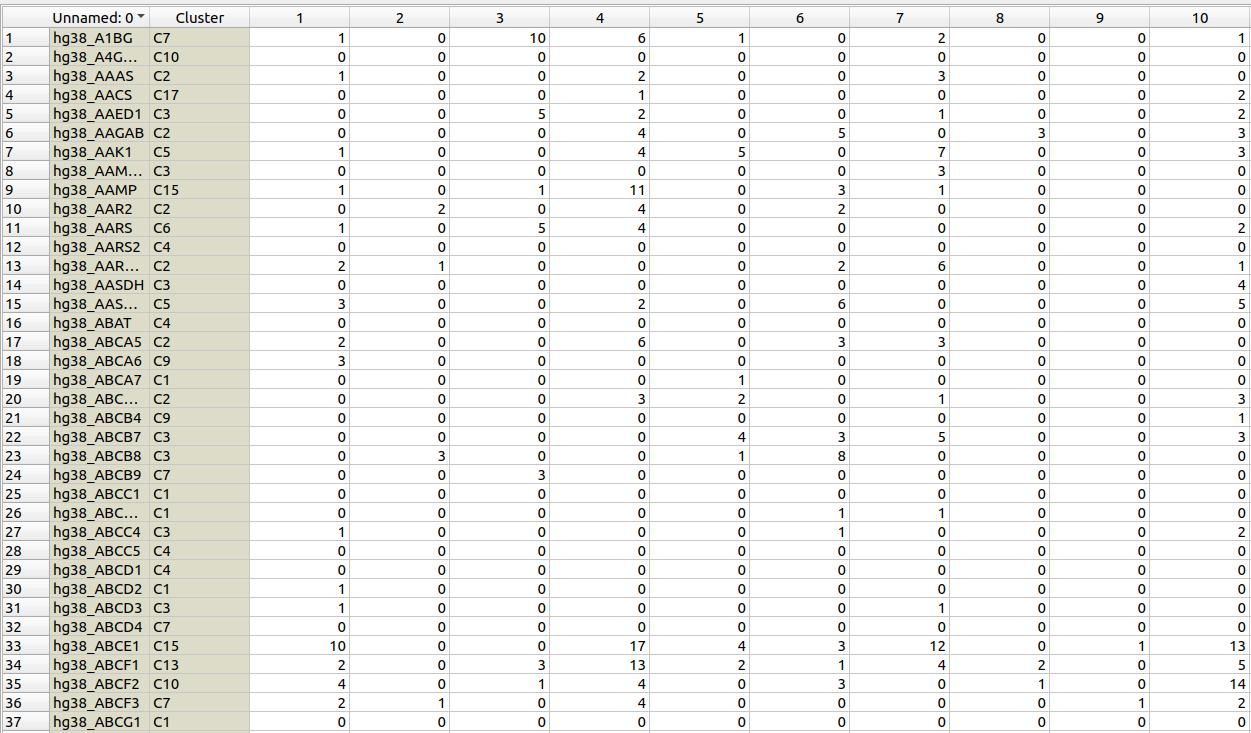
\includegraphics[width=12cm]{images/louvian_clusters_18_euclidan.png}}}}
\caption{19 klastera}
\end{figure}  

Veličine klastera:
\begin{tcolorbox}
\begin{verbatim}
C0: 1098
C1: 1093
C2: 956
C3: 954
C4: 843
C5: 806
C6: 699
C7: 631
C8: 595
C9: 537
C10: 491
C11: 480
C12: 399
C13: 359
C14: 178
C15: 156
C16: 112
C17: 91
C18: 83
\end{verbatim}
\end{tcolorbox}
    
\\    

\begin{figure}[H]
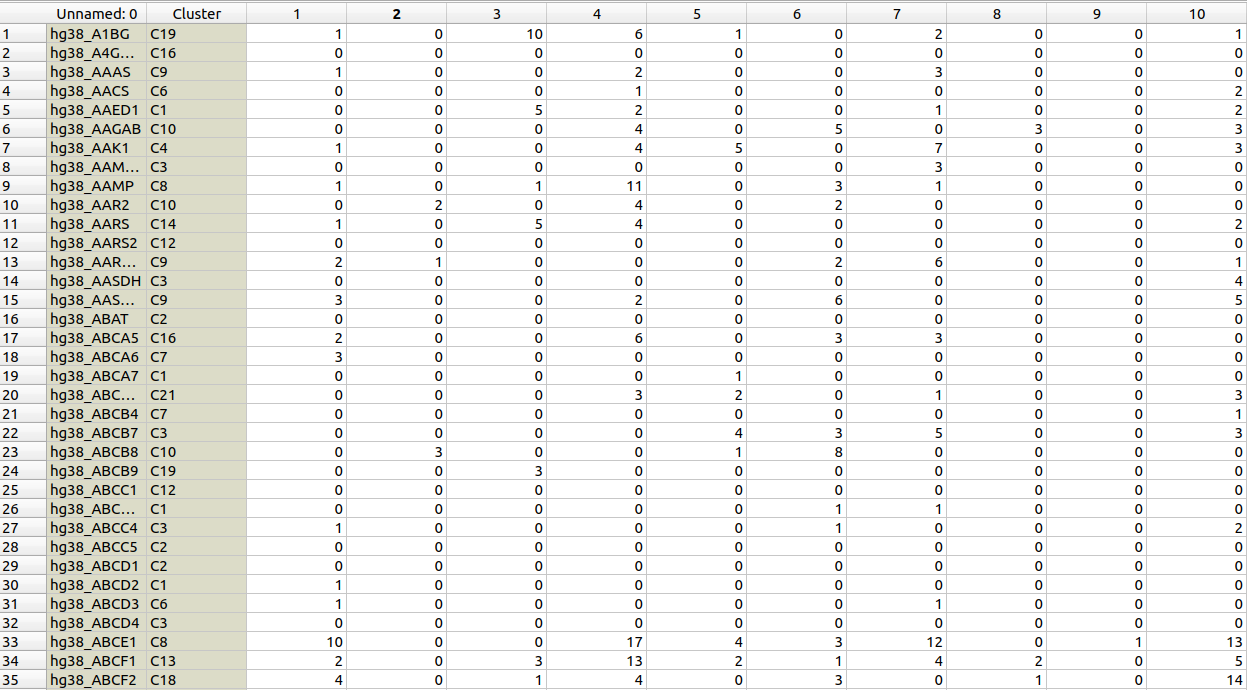
\includegraphics[width=12cm]{images/manhatn_24_clusters.png}}}}
\caption{10 klastera}
\end{figure}  

\begin{tcolorbox}
\begin{verbatim}
C0: 9%
C1: 9%
C2: 10%
C3: 11%
C4: 6%
C5: 9%
C6: 9%
C7: 12%
C8: 16%
C9: 9%
\end{verbatim}
\end{tcolorbox}

Iz dobijenih rezultata može se zakjučiti da Louvian metod klasterovanja postiže zadovoljavajuće rezultate. U slučaju klasterovanja podataka u 19 klastera, podaci nisu sasvim ravnomerno raspoređeni, dok su u slučaju povećanja parametra \textbf{resolution} izdvaja 10 klastera približno slične veličine. Klasterovanje je vršeno koristeći Menhetn i Euklidsko rastojanje, pri čemu nije bilo značajnije razlike između ove dve metode.
Takođe, valja napomenuti da je u softveru Orange ispis nakon klasterovanja moguć samo u okviru tabele, odnosno nije moguće grupisati nazive dobijenih gena, stoga su pomoću siluete date veličine i rastojanja između klastera, kao i skica same tabele.


\subsubsection{Klasterovanje ćelija}

\begin{figure}[H]
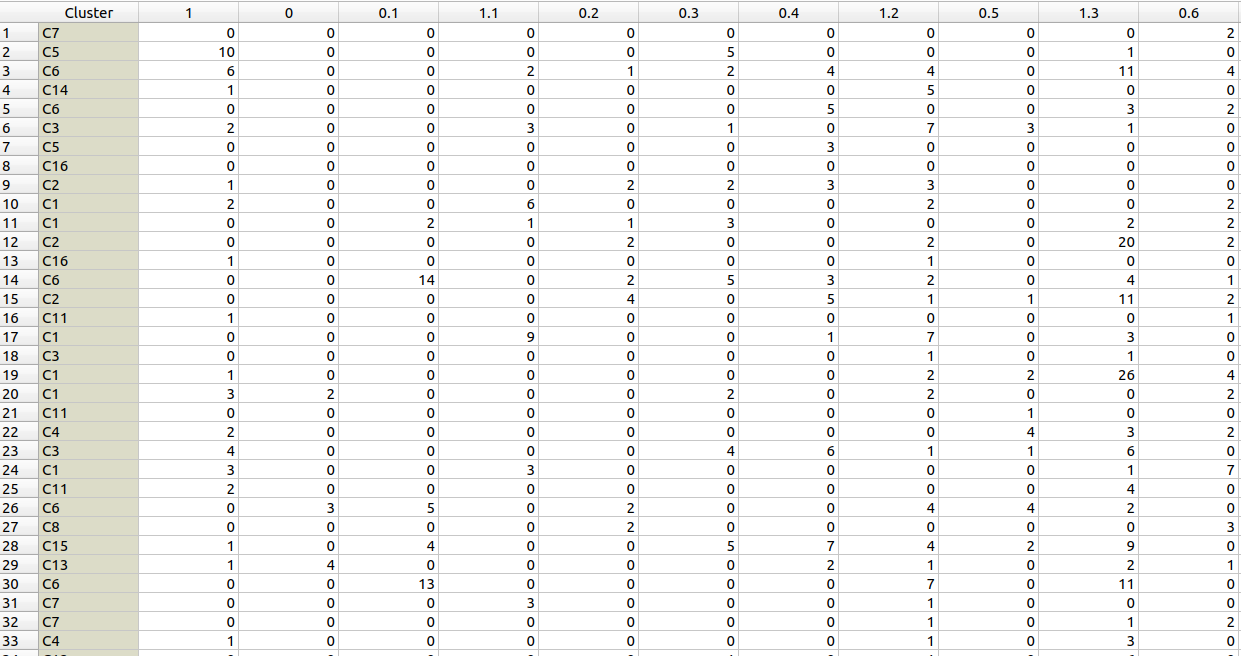
\includegraphics[width=12cm]{images/louviane_cells.png}}}}
\caption{10 klastera}
\end{figure}  
 
\\
\begin{tcolorbox}
\begin{verbatim}
C0: 7%
C1: 6%
C2: 10%
C3: 12%
C4: 10%
C5: 10%
C6: 11%
C7: 11%
C8: 10%
C9: 13%
\end{verbatim}
\end{tcolorbox} 
 
 
\section{CLARA}
\textbf{CLARA}(Clustering Large Applications) je algoritam koji predstavlja nadogradnju alogritma \textbf{k-medioida}, u cilju brže obrade velikih skupova podataka.
Za razliku od klasičnog algoritma k-medioda koji računa medioide za kompletan skup podataka, \textbf{CLARA} u obzir uzima mali uzorak skupa fiksirane veličine na koji primenjuje \textbf{PAM} algoritam izračunavajući tako optimalan skup medioida.
Kako se u procesu računanja ne koristi kompletan skup, dobijeni rezultati se mogu značajno razlikovati od stvarnih, ipak \textbf{CLARA} ponavalja proces slučajnog pronalaženja uzorka i primene \textbf{PAM} algoritma nad istim čime se minimizuje greška. Implementacija algoritma data je u programskom jeziku R.

\\

Neophodno je instalirati pakete \textit{factoextra} i \textit{cluster}. Navedeno se može uraditi naredbama:

\begin{tcolorbox}
\begin{verbatim}
install.packages("factoextra")
install.packages("cluster")
\end{verbatim}
\end{tcolorbox}

a potom iste i učitati:

\begin{tcolorbox}
\begin{verbatim}
library(factoextra)
library(cluster)
\end{verbatim}
\end{tcolorbox}



\begin{tcolorbox}
\begin{verbatim}
 dataset = read.csv(header = FALSE, sep = ",", 
            file = "data.txt")

head(dataset, nrows = 3)
x = as.matrix(sapply(dataset, as.numeric)) 


fviz_nbclust(x = dataset, FUNcluster = clara, 
            method = "silhouette", 
            diss = NULL, k.max = 10, nboot = 100, 
            verbose = interactive(), 
            barfill = "steelblue", barcolor = "steelblue", 
            linecolor = "steelblue", print.summary = TRUE)

clara.results = clara(x, 4, samples = 50, pamLike = TRUE)
print(clara.results)

fviz_cluster(clara.results, data = NULL, choose.vars = NULL, 
                stand = TRUE,   axes = c(1, 2), 
                geom = c("point", "text"),
                repel = FALSE,
                show.clust.cent = TRUE, ellipse = TRUE, 
                ellipse.type = "convex",
                ellipse.level = 0.95, \
                ellipse.alpha = 0.2, shape = NULL,
                pointsize = 1.5, labelsize = 12, 
                main = "Cluster plot", xlab = NULL,
                ylab = NULL, outlier.color = "black", 
                outlier.shape = 19,
                ggtheme = theme_grey())


\end{verbatim}
\end{tcolorbox}

\\
Nakon učitavanja skupa podataka, iste je neophodno pretvoriti u numeričku matricu koja predstavlja ulaz za \textbf{CLARA} algoritam.
Pre samog procesa klasterovanja, poželjno je odrediti optimalan broj klastera.
\\
Navedeno se može uraditi funkcijom \textit{fviz\_nbclust} iz paketa \textit{factoextra}.

\begin{itemize}
    \item x - ulazni skup podataka
    \item FUNCluster - algoritam klasterovanja
    \item method - mera koja se koristi za određivanje broj klastera
    \item k.max - maksimalan broj klastera
    \item nboot - broj iteracija
\end{itemize}



\subsubsection{Klasterovanje gena}
Prilikom klaterovanja gena korišćen je pripremljeni skup podataka. Primenom funkcije za određivanje broja klastera, grafik dostiže maksimalnu vrednost za ulazne parametre 2 i 7, što implicira da podatke treba podeliti u 2, odnosno 7 klastera.


\begin{figure}[H]
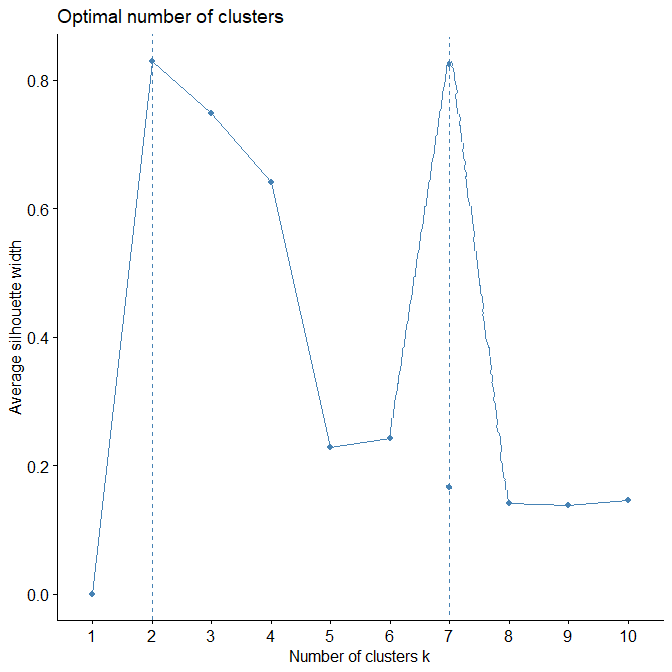
\includegraphics[width=12cm]{images/numberOfClustersGenesmade.png}}}}
\caption{rezultat primene funkcije fviz\_nbclust}
\end{figure} 

 


\begin{figure}[H]
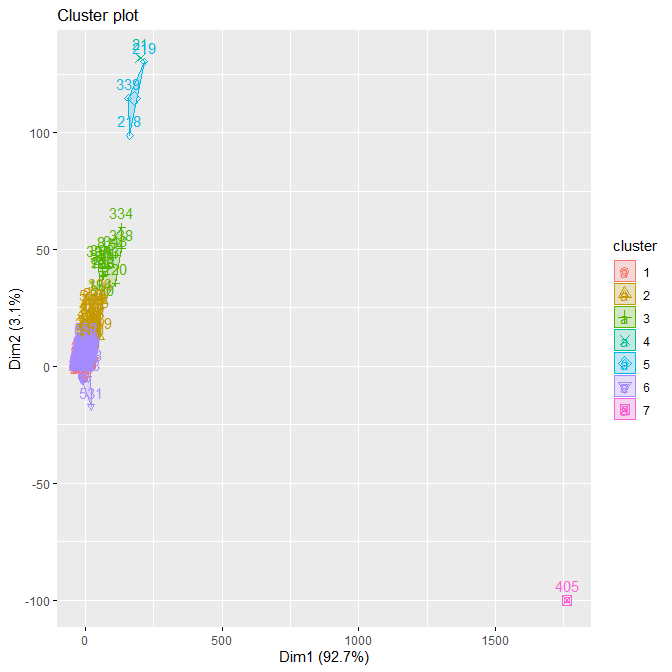
\includegraphics[width=12cm]{images/ploting.png}}}}
\caption{vizualizacija dobijenih klastera}
\end{figure} 

Klasterovanje sa ovakvim parametrima rezultiralo je prilično ujednačenim klasterima, međutim prilikom grupisanja podataka u 7 klastera jasno su bila vidljiva određena preklapanja među klasterima, tako da na slici nije moguće jasno utvrditi granice između klastera, čak su i pojedini klasteri usled preklapanja nevidljivi.
\\

\begin{tcolorbox}
\begin{verbatim}
Objective function: 308.2523
Clustering vector: int [1:10561] 1 1 1 2 1 2 3 1 4 5 1 5 1...
Cluster sizes: 1321 1041 312 2235 2002 850 3700
\end{verbatim}
\end{tcolorbox}


\subsubsection{Klasterovanje ćelija}
Za klasterovanje ćelija, kao i u prethodnim slučajevima, biće iskorišćeni transponovani podaci.
Izračunat je optimalan broj klastera i on iznosi dva, međutim, kako su i ostale vrednosti(u rasponu od 1 do 10) imale sličnu vrednost algoritam je primenjen za različite vrednosti broja klastera.

\begin{figure}[H]
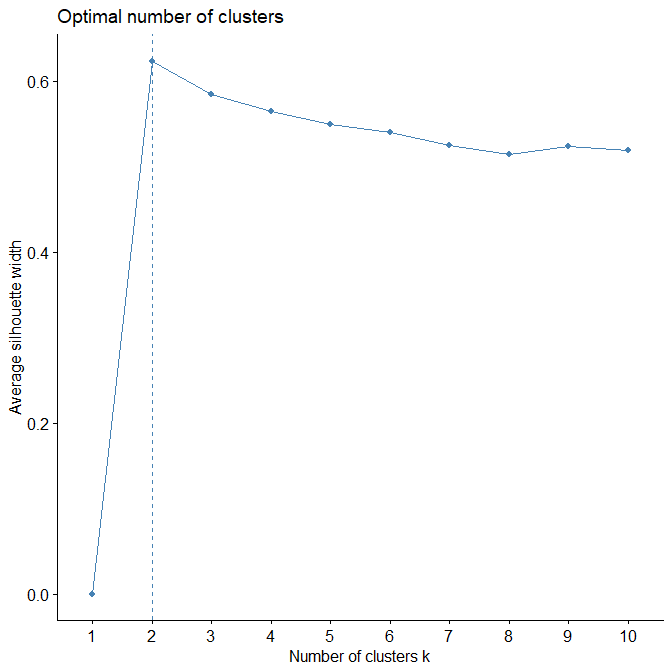
\includegraphics[width=12cm]{images/numbercells.png}}}}
\caption{rezultat primene funkcije fviz\_nbclust}
\end{figure} 

\begin{figure}[H]
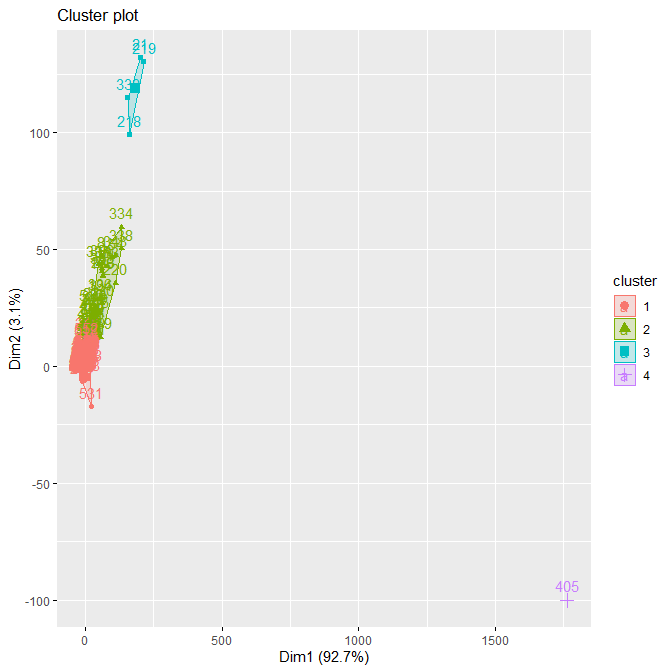
\includegraphics[width=12cm]{images/clusters.png}}}}
\caption{vizualizacija dobijenih klastera}
\end{figure} 

Klasterovanje ćelija u slučaju 4 klastera dalo je povoljne rezultate. Klasteri su dobro grupisani, i sličnih veličina, s tim što se jedan klaster tretirao kao elementi van granica. 
\begin{tcolorbox}
\begin{verbatim}
Objective function: 14.531
Clustering vector: int [1:6484] 12 2 1 2 3 2 3 4 1 1 1 1 1 2...
Cluster sizes: 1609 x 1918 2957
\end{verbatim}
\end{tcolorbox}



\section{Algoritam DBSCAN}
\label{sec:specijalni slucajevi}
 

\textbf{DBSCAN} algoritam predstavlja klasterovanje zasnovano na gustini, odnosno, prepoznaje regione visoke gustine koji su međusobno razdvojeni regionima niske gustine. Gustina se definiše kao broj tačaka u okviru određenog poluprečnika(\textit{eps}).
DBSCAN može da prepoznaje klastere različitih oblika i gustina. Odabirom različitih vrednosti za parametre \textit{eps} i \textit{minPts} mogu se pogodno prepoznati klasteri određene gustine, međutim u tom slučaju drugi(retki) klasteri mogu izgledati kao šum.
\\
 
\begin{figure}[H]
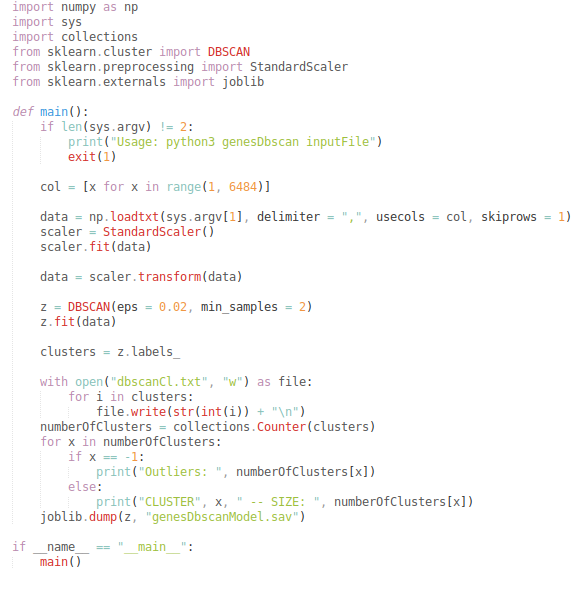
\includegraphics[width=12cm]{images/dbscanpy.png}}}}
\caption{implementacija DBSCAN algoritma}
\end{figure}  



\\
\subsection{Klasterovanje gena}
Klasterovanje algoritmom DBSCAN nije dalo željene rezultate. Uprkos definisanju različitih vrendosti za parametre \textit{eps} i \textit{minpts}, sve vrednosti su bile predstavljene kao elementi van granica iz čega zaključujemo da ovaj algoritam zasnovan na gustini nije pogodan za klasterovanje ovakvog tipa podataka.
U nastavku su prikazani rezultati za različite vrednosti parametara \textit{eps} i \textit{minPts}.
\\

\begin{tcolorbox}
\begin{verbatim}
  Eps = 0.7
  MinPts = 14
 
  Outliers:   10561
\end{verbatim}
\end{tcolorbox}

\begin{tcolorbox}
\begin{verbatim}
  Eps = 0.4
  MinPts = 11
  
  CLUSTER0 -- SIZE: 14
  CLUSTER1 -- SIZE: 25
  CLUSTER2 -- SIZE: 11
  CLUSTER3 -- SIZE: 7
  
  Outliers:   10504
\end{verbatim}
\end{tcolorbox}


\begin{tcolorbox}
\begin{verbatim}
  Eps = 0.3
  MinPts = 9
 
  Outliers:   10561
\end{verbatim}
\end{tcolorbox}

\begin{tcolorbox}
\begin{verbatim}
  Eps = 0.1
  MinPts = 5
 
  Outliers:   10561
\end{verbatim}
\end{tcolorbox}

\begin{tcolorbox}
\begin{verbatim}
  Eps = 0.02
  MinPts = 2
 
  Outliers:   10561
 
\end{verbatim}
\end{tcolorbox}
 

 

\section{Klasterovanje metodom K-means}
Klasterovanje metodom \textbf{K-means} predstavlja metod za analizu grupisanja koja za cilj ima podelu objekata u \textbf{k} klastera, pri čemu svaki objekat pripada klasteru sa najsličnijim osobinama. Klasterovanje će biti vršeno u programskom jeziku Python, uz pomoć bibiloteka \textit{sklearn, pandas, numpy, matplotlib}.


 


\subsection{Klasterovanje gena}
Pre početka procesa klasterovanja, kao i u slučaju \textbf{CLARA} algoritma, najpre je neophodno odrediti optimalan broj klastera. Broj klastera moguće je odrediti na osnovu vrednosti \textit{inertia}. Kako bi se pristupilo datoj promenljivoj, izvršićemo najpre klasterovanje za vrednosti \textbf{k} u opsegu 1-20 nakon čega ćemo odrediti optimalan broj klastera.


\begin{figure}[H]
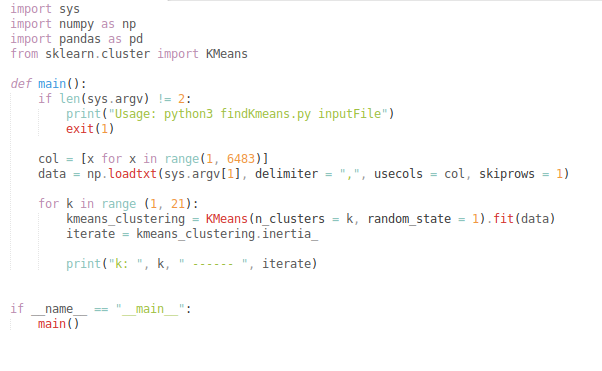
\includegraphics[width=12cm]{images/kmeansFind.png}}
\caption{findKmeans.py}
\end{figure}


Pozivom programa iznad dobijamo sledeći rezultat.

\begin{tcolorbox}
\begin{verbatim}
k:  1  ------  112468838126.22235
k:  2  ------  52403795184.77562
k:  3  ------  25666530479.058987
k:  4  ------  17245417713.175568
k:  5  ------  14139942030.161459
k:  6  ------  11997712819.261986
k:  7  ------  10914223612.17275
k:  8  ------  9964115336.273674
k:  9  ------  9277906309.844564
k:  10  ------  8581792905.926445
k:  11  ------  8010461744.837661
k:  12  ------  7176757398.016832
k:  13  ------  6836614168.836437
k:  14  ------  6308053233.808801
k:  15  ------  5989325457.669791
k:  16  ------  5376111680.354345
k:  17  ------  5169671282.9423895
k:  18  ------  4814736658.926268
k:  19  ------  4664123191.664272
k:  20  ------  4426681029.103273

\end{verbatim}
\end{tcolorbox}

\\

Vrednost cost dobijamo pomoću promenljive inertia koja predstavlja sumu
kvadratnih rastojanja uzoraka do njihovih najbližih centroida. Trebalo bi da se k
izabere u trenutku kada vrednost cost prestane da se razlikuje značajno. Vrednost
cost se ne menja značajno kada se za k uzimaju vrednosti od 12 do 17, pa će broj
klastera biti 15, jer predstavlja sredinu intervala kada je vrednost cost prestala naglo da opada. Sada kada znamo na koliko klastera ćemo klasterovati podatke pokrenućemo klasterovanje metodom K-means.

\begin{figure}[H]
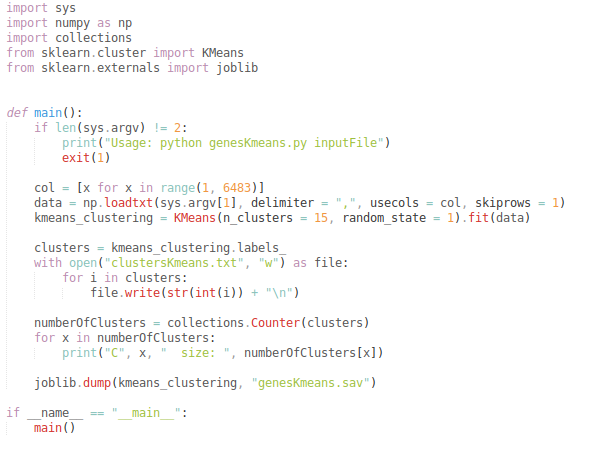
\includegraphics[width=12cm]{images/kmeansGenes.png}}
\caption{genesKmeans.py}
\end{figure}

Rezultati koje smo dobili dati su u sledećoj tabeli.

\begin{tcolorbox}
\begin{verbatim}
C 0   size:  9872
C 5   size:  533
C 11   size:  1
C 1   size:  35
C 4   size:  65
C 9   size:  12
C 3   size:  1
C 6   size:  2
C 12   size:  1
C 8   size:  1
C 10   size:  3
C 13   size:  27
C 7   size:  5
C 14   size:  2
C 2   size:  1

\end{verbatim}
\end{tcolorbox}

\\

Iz priloženih rezultata vidimo da klasteri nisu ravnomerno raspoređeni, te stoga zaključujemo da metoda \textbf{K-means} ne uspeva dovoljno dobro da klasteruje gene.

\\

\subsection{Klasterovanje ćelija} 
U slučaju klasterovanja ćelija koristićemo transponovane podatke.

\begin{figure}[H]
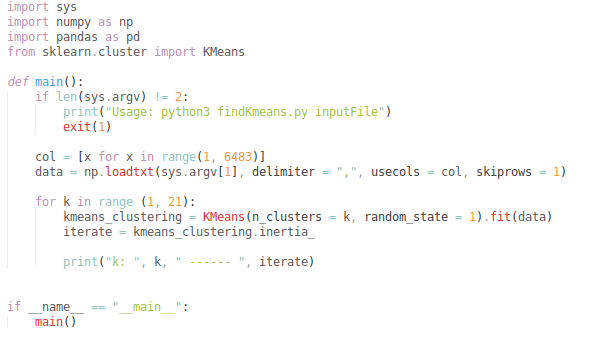
\includegraphics[width=12cm]{images/kmeansCells.png}}
\caption{cellsKmeans.py}
\end{figure}

Rezultati koje smo dobili dati su u sledećoj tabeli.

\begin{tcolorbox}
\begin{verbatim}
Cid:     8  Size:   530
Cid:     0  Size:  1037
Cid:    14  Size:   493
Cid:     3  Size:   281
Cid:     7  Size:   426
Cid:     1  Size:   289
Cid:    12  Size:   880
Cid:    13  Size:   131
Cid:     4  Size:   722
Cid:     6  Size:   725
Cid:    11  Size:   251
Cid:    10  Size:   571
Cid:     5  Size:    41
Cid:     9  Size:    90
Cid:     2  Size:    16
\end{verbatim}
\end{tcolorbox}

\\

Kod klasterovanja ćelija podaci su ravnomernije raspoređeni u klastere u odnosu
na klasterovanje gena.
\\

\section{Hijerarhijsko klasterovanje}
Hijerarhijsko klasterovanje jedna je od osnovnih tehnika klasterovanja, koja iako staromodna, i dalje široko rasprostranjena. U slučaju ovakvog pristupa, nema potrebe za određivanjem broja klastera. Hijerahijsko klasterovanje se često grafički prikazuje u obliku drveta koje se naziva dendrogram. \textbf{Dendrogram} pokazuje klastere i podklastere. Željeni broj klastera ostvaruje se skraćivanjem dendrograma, odnosno sečenjem dobijenog drveta. 
U osnovi, postoje dva tipa ovakvog klasterovanja:
\begin{itemize}
\item Sakupljajuće - polazi se od činjenice da svaka tačka predstavlja jedan klaster, nakon čega se spajaju po dve najbliže tačke sve dok se ne dođe do 1 ili k klastera
\item  Razdvajajuće - polazi se od jednog velikog klastera, nakon čega se isti razbija sve dok se ne dođe do 1 ili k klastera
\end{itemize}



\subsection{Klasterovanje gena}
Pre klasterovanja podataka, odredićemo broj klastera. Optimalan broj klastera biće određen grafičkim putem, pomoću dendrograma.
\\
\\ \\ 





\begin{figure}[H]
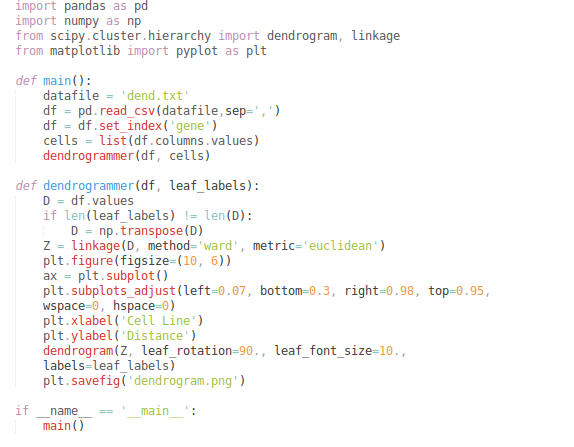
\includegraphics[width=12cm]{images/dendrogram.png}}}}
\caption{dendrogram}
\end{figure}

Biće prikazana različita rešenja, gde će biti promenjen broj klastera, mera sličnosti i metode povezivanja.
Najčešće se koristi \textbf{Lance-Vilijamsova} grupa metoda:
\begin{itemize}
\item Single linkage - mera rastojanja između dva klastera predstavlja
minimalno rastojanje između parova obekata koji pripadaju ovim klasterima.
\item Complete linkage - rastojanje između dva klastera predstavlja
maksimalno rastojanje između parova objekata koji pripadaju tim klasterima.
\item Average linkage - rastojanje se određuje prema prosečnom rastojanju svih objekata koji pripadaju dvema grupama.
\item Ward - poznata i kao metoda minimalne varijanse. Kao i ostale metode
povezivanja, kreće se od m klastera (svaki klaster sadrži jedan objekat),
ali se ne računa udaljenost između klastera, već se maksimizira homogenost
unutar klastera. Ukupna suma kvadrata unutar klastera (SSE) se računa u
cilju utvrđivanja koje se dve grupe spajaju u svakom koraku algoritma. 
\end{itemize}


\begin{figure}[H]
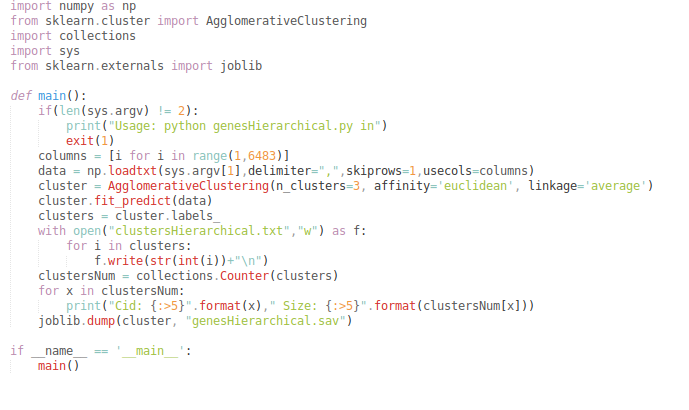
\includegraphics[width=12cm]{images/hierargenes.png}}}}
\caption{genesHierarchical.py}
\end{figure}

U nastavku će biti izloženi rezultati klasterovanja za različite parametre.


\begin{tcolorbox}
\begin{verbatim}
Cid:     4  Size: 10486
Cid:    11  Size:     1
Cid:     7  Size:     1
Cid:     0  Size:    57
Cid:    13  Size:     1
Cid:    12  Size:     1
Cid:     9  Size:     1
Cid:     5  Size:     1
Cid:     8  Size:     1
Cid:     3  Size:     1
Cid:     1  Size:     3
Cid:     2  Size:     5
Cid:     6  Size:     1
Cid:    10  Size:     1

\end{verbatim}
\end{tcolorbox}

\begin{tcolorbox}
\begin{verbatim}
Cid:     2  Size: 10549
Cid:     0  Size:    11
Cid:     1  Size:     1    
\end{verbatim}
\end{tcolorbox}



Klasterovanje prosečnom vezom, pri čemu je broj klastera postavljen na 14 nije dalo željene rezultate. Jedan klaster sadrži ogromnu većinu podataka, dok se u preostalih 13 klastera nalazi minimalan broj istih. Stoga možemo zaključiti da ovakvi parametri nisu pogodni za klasterovanje datih gena. Slična situacija je bila i u slučaju 3 klastera.

\\

\begin{tcolorbox}
\begin{verbatim}
Cid:     1  Size: 5256
Cid:     2  Size: 970
Cid:     0  Size: 4355

\end{verbatim}
\end{tcolorbox}

Ward metodotom dobijeni su značajno bolji rezultati. Izdvojena su tri klastera, međutim podaci nisu i dalje u potpunosti ravnomerno raspoređeni.

\begin{tcolorbox}
\begin{verbatim}
Cid:     0  Size: 10551
Cid:     2  Size:     9
Cid:     1  Size:     1
\end{verbatim}
\end{tcolorbox}

Rezultati dobijeni za kompletnu vezu.


 

\subsection{Klasterovanje ćelija}
Kao i kod metode K-means koristićemo iste transponovane podatke.

\begin{figure}[H]
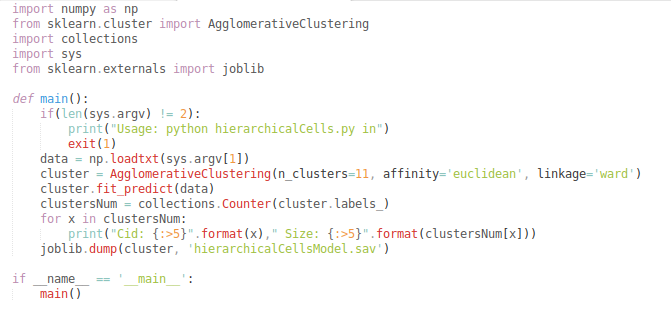
\includegraphics[width=12cm]{images/hierarcells.png}}}}
\caption{cellsHierarchical.py}
\end{figure}


\begin{tcolorbox}
\begin{verbatim}
Cid:     8  Size:   642
Cid:     3  Size:  1796
Cid:     2  Size:   329
Cid:     4  Size:   409
Cid:     5  Size:   534
Cid:     7  Size:   868
Cid:    10  Size:   410
Cid:     6  Size:   744
Cid:     9  Size:   559
Cid:     0  Size:   159
Cid:     1  Size:    33

\end{verbatim}
\end{tcolorbox}

Ward metod dao je zadovoljavajuće rezultate u slučaju klasterovanja ćeija. Podaci su ravnomerno raspoređeni, klasteri su slične veličine izuzev dva klastera koja odstupaju od ostatka.

\begin{tcolorbox}
\begin{verbatim}
Cid:     1  Size:  6421
Cid:     7  Size:    45
Cid:     0  Size:     8
Cid:     3  Size:     4
Cid:     2  Size:     2
Cid:     5  Size:     1
Cid:     6  Size:     1
Cid:     4  Size:     1
\end{verbatim}
\end{tcolorbox}

Rezultati za prosečnu vezu i 8 klastera. Podaci su velikom većinom grupisani u jedan klaster, dok ostatak grupa sadrži izuzetno mali broj podataka.


\section{Samoorganizujuće mape}
 
Samoorganizujuća mapa predstavlja tip veštačke neuronske
mreže čija obuka se vrši nenadgledanim učenjem kako bi se dobila niskodimenzionalna
reprezentacija ulaznih uzoraka.
Samoorganizujuće mape razlikuju se od drugih tipova neuronskih mreža po tome što čuvajuinformaciju o
topološkim svojstvima ulaza pomoću funkcije susednih neurona.
\\
\\
Rad samoorganizujućih mapa sastoji se iz dve faze: 
    \begin{itemize}
        \item faza učenja - izgrađuje se mapa pomoću ulaznih podataka
        \item faya preslikavanja - vrši se klasifikacija ulaznog vektora
    \end{itemize}
\\

Samoorganizujuća mapa sastoji se iz čvorova, odnosno nerona. Svaki neuron definisan je svojim vektorom težina, pri čemu isti mora biti iste dimenzije kao i ulazni vektor podataka. Proces smeštanja vektora iz prostora podataka u mapu sastoji se iz pronalaženja neurona čiji vektor težina ima vrednosti najbliže vektoru iz prostora podataka, nakon čega sledi dodeljivanja koordinata mape neurona odgovarajućem vektoru.    

 
 
\begin{figure}[H]
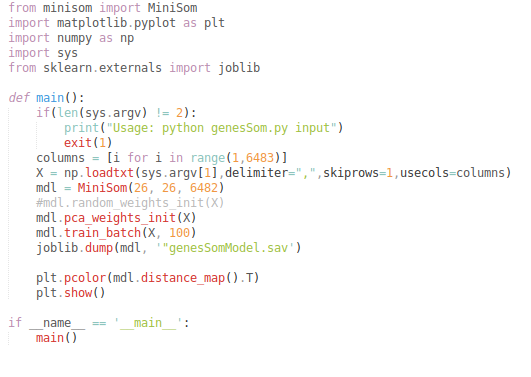
\includegraphics[width=12cm]{images/ge.png}}}}
\caption{genesSom.py}
\end{figure}

\\

Dimenzija matrice (mape) kod samoorganizujućih mapa dobija se po formuli:
     \begin{equation}\label{neurform} M^2 \approx 5\sqrt{N},\end{equation}
de je M broj neurona, koji predstavlja ceo broj blizak jednačini sa desne strane,
gde je N broj objekata.
Samoorganizujuća mapa će biti korišćena radi vizuelizacije podataka nakon čega
ćemo moći preko toplotnih mapa da zaključimo broj klastera. U implementaciji
samoorganizujućih mapa u na dva načina se mogu podaci uzimati
iz skupa, prvi je nasumičnim izborom gde se koristi metoda \textbf{trainrandom} a
drugi je sekvencijalno, odnosno podaci se uzimaju redom gde se koristi metoda \textbf{trainbatch}.
 



 
\begin{figure}[H]
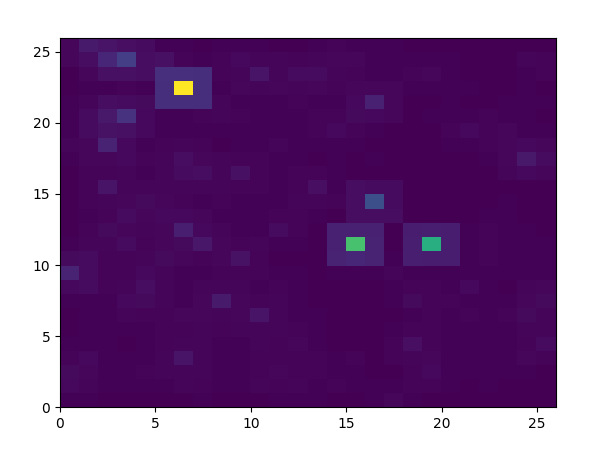
\includegraphics[width=12cm]{images/random_genes.png}}}}
\caption{Toplotna mapa dobijena nasumičnim izborom gena}
\end{figure}
Izdvojena su četiri skupa podataka, pri čemu ostatak podataka nije prepoznat ovakvim nasumičnim izborom gena. Sa ovako dobijene mape moglo bi se pretpostaviti da podatke treba podeliti u četiri klastera, međutim upitne su veličine istih, jer veliki broj podataka nije u potpunosti uočen.

\begin{figure}[H]
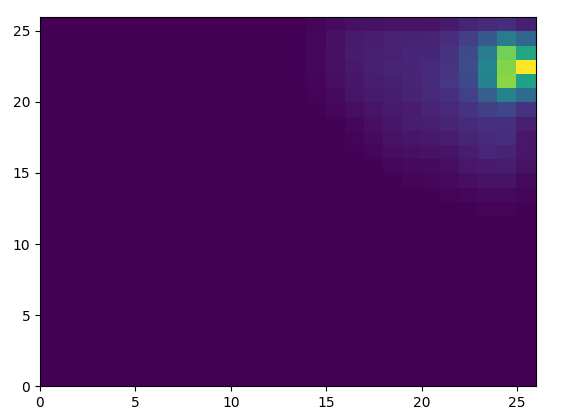
\includegraphics[width=12cm]{images/not_random.png}}}}
\caption{Toplotna mapa dobijena izborom gena po redosledu}
\end{figure}
Određeni broj podataka grupisan je zajedno u jednu grupu dok ostatak podataka nije prepoznat u ovom slučaju.

\begin{figure}[H]
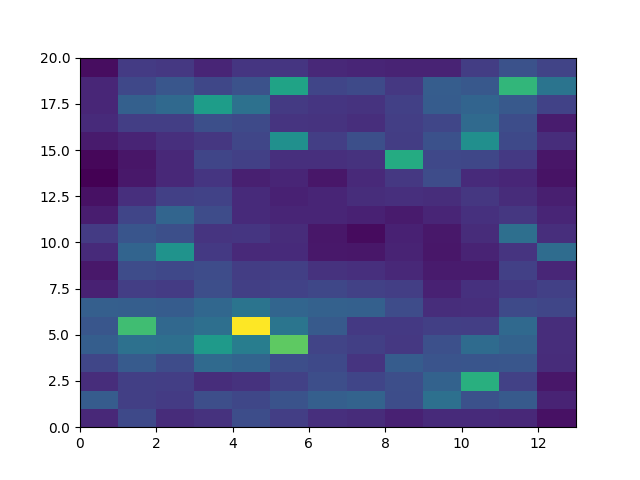
\includegraphics[width=12cm]{images/cellsSomRandom.png}}}}
\caption{Toplotna mapa dobijena nasumičnim izborom ćelija}
\end{figure}
Kako se može videti sa dobijene mape, podatke bi bilo pravilno rasporediti u četiri klastera, pri čemu su isti sličnih veličina. Takođe postoji i određeni broj podataka koji se nalazi između dva ili više klastera te stoga mogu biti u sastavu više od jednog klastera.

\begin{figure}[H]
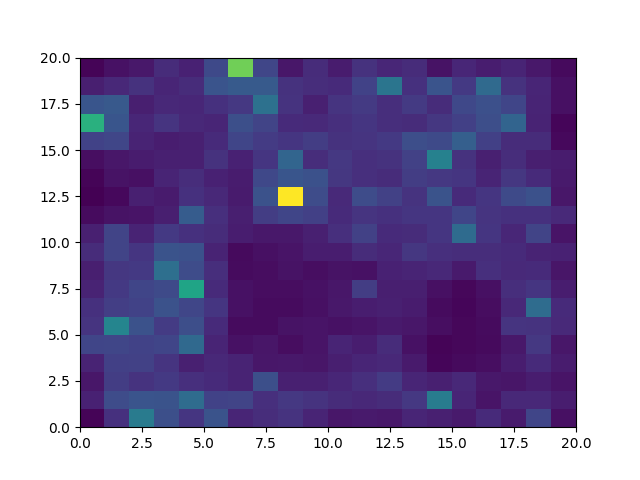
\includegraphics[width=12cm]{images/cellsSomRandom2.png}}}}
\caption{Toplotna mapa dobijena nasumičnim izborom ćelija}
\end{figure}

Sa date slike može se videti da su podaci rasuti po mapi i da nisu kvalitetnu grupisani
u klastere.


\section{Zaključak}
\\ Modeli algoritama koji su implementirani u programskom jeziku Python sačuvani su u direktorijumu \textbf{models}, sa odgovarajućim nazivom. Isti se mogu učitati komandom \textit{joblib.load(ime\_fajla)}.
Rešenja koja su dobijena, odnosno raspored ćelija i gena po klasterima nalaze se u direktorijumu \textbf{clusters}, sačuvana kao txt datoteke odgovarajućeg naziva.
U istom direktorijumu nalaze se i dobijene toplotne mape.
\\

Nakon primene različitih metoda i tehnika, možemo zaključiti da ulazni skup podataka nije u potpunosti pogodan za klasterovanje. U okviru klasterovanja gena, poželjne rezultate postigli smo klasterovanjem CLARA algoritmom, nešto lošiji bili su rezultati primene Louviane metode, dok se ostale tehnike nisu pokazale dobro. Slučaj klasterovanja ćelija bio je nešto efikasniji, pa se kvalitetan raspored podataka postigao u većem broju slučajeva.
U sledećoj tabeli date su procene kvaliteta klasterovanja različitim metodama zasnovane na \textbf{Davis-Bouldinovom} indeksu.
\\
\textbf{Davis-Bouldinov} indeks definiše se kao prosečna sličnost između svakog klastera sa klasterom koji mu je najsličniji.

\\

$$ DB = \frac{1}{k}\sum max_{i\neq j}R_{ij} $$

gde je:
    $$ R_{ij} = \frac{s_{i}+s_{j}}{d_{ij}} $$

\begin{itemize}
    \item $s_{i}$ - prosečno rastojanje tačaka klastera od centra istog
    \item $d_{ij}$ - rastojanje između centara klastera \textit{i} i \textit{j}
\end{itemize}


\begin{center}
 \begin{tabular}{||c c c c c||} 
 \hline
 K-means & DBSCAN & H - Average & H - Single & H - Ward \\ [0.5ex] 
 \hline\hline
 0.78 & 1.89 & 0.3 & 0.47 & 0.4 \\ 
 \hline
\caption{\label{tab:table-name}KLASTEROVANJE GENA}
\end{tabular}
\end{center}

Kako su kvalitet razdvojenosti klastera i Davis-Bouldinov indeks obrnuto proporcionalni, odnosno, veća vrednost indeksa označava i lošiji kvalitet klasterovanja, zaključujemo da su se u slučaju klasterovanja gena najbolje pokazao algoritam Hijerarhijskog klasterovanja, pri čemu su rezultati najbolji za prosečnu vezu. DBSCAN algoritam očekivano ima najlošije rezultate.

\\

\begin{center}
 \begin{tabular}{||c c c c||} 
 \hline
 K-means & H - Average & H - Single & H - Ward \\ [0.5ex] 
 \hline\hline
 1.68 & 0.2 & 0.3 & 0.44\\ 
 \hline
\caption{\label{tab:table-name}KLASTEROVANJE ĆELIJA}
\end{tabular}
\end{center}

Kao i u slučaju klasterovanja gena, prilikom klasterovanja ćelija najbolji rezultati ponovo su dobijeni hijerarhijskim klasterovanjem. Sa druge strane, algoritam k-means, iako je na prvi pogled dao kvalitetne rezultate prilikom grupisanja ćelija ipak ima lošiji DB indeks.

\\

Važno je napomenuti da se rezultati navedeni u prethodne dve tabele odnose na algoritme klasterovanja koji su implementirani u programskom jeziku Python, takođe kako su prilikom klasterovanja korišćeni različiti parametri u tabeli su navedeni samo najbolji rezultati za svaku od tehnika. Kako softver Orange ne raspolaže testovima koji bi odredili kvalitet klasterovanja, rezultati primenjenih tehnika u istom dati su u vidu slika koje se odnose na veličinu dobijenih klastera.



\begin{thebibliography}{9}

\bibitem{intr} 
Introduction to data mining\\
Pang-ning Tan and Michael Steinbach and Vipin Kumar, 2005

\bibitem{stanford} 
Clustering Algorithms in data mining\\
Jure Leskovec and Anand Rajaraman, Stanford Univeristy
 
\bibitem{datanovia} 
Datanovia: Data Analysis and Visualization 
 
\bibitem{skitlearn}
Skit-learn library
\\\texttt{https://scikit-learn.org}

\bibitem{orange}
Orange Data Mining Software
\\\texttt{https://https://orange.biolab.si/}
 
\bibitem{neo4j} 
Neo4J: Graph Algorithms
\\\texttt{https://neo4j.com/docs/graph-algorithms/current/algorithms/louvain/}
\end{thebibliography}

\end{document}
